% !TeX spellcheck = en_GB
% !TeX root = Report.tex

\phantomsection
\addcontentsline{toc}{section}{Introduction}
\sect{Introduction to Governance}

Government legislation pervades all aspects of modern life from welfare to industry, infrastructure to enterprise.
This report is primarily concerned with legislation that governs industry.
Finance, healthcare and research are just a few areas that are subject to government legislation.
Large national infrastructure such as energy, transport, water and communication are also particularly heavily regulated.
In this report, the role of governance in several industries is examined to understand how legislation can promote or diminish the profit potential of technology dependent industries.

The dictionary definition of legislation is ``laws, considered collectively'' \cite{OED} and the two terms are used synonymously in this report.
One of the main roles of the elected parliament is the debate and passing of new laws or modification to laws.
Figure \ref{figure:passage} shows how new legislation comes into being through the parliamentary process.

\begin{figure}[!h]
\centering
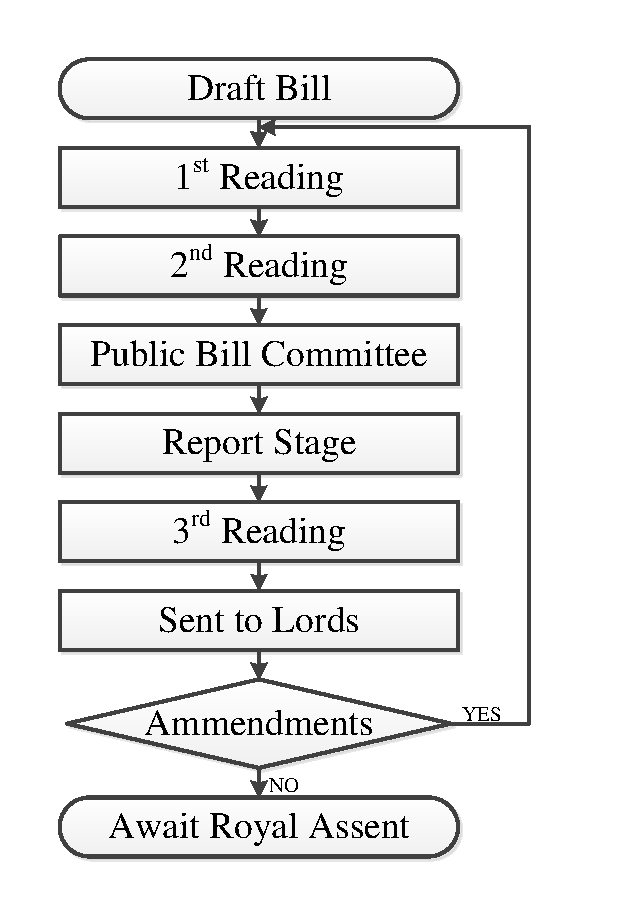
\includegraphics[width = 0.27\textwidth]{Figures/BillFormulation.pdf}
\caption{The passage of a Bill or Act to become Law - adapted from \cite{Factsheet2010}}
\label{figure:passage}
\end{figure}

The legislation the government sets influences industry in two ways; directly or indirectly.
Direct investment in infrastructure is one method the government uses to establish infrastructure.
Historically, this has been the case for many of the then privatised industries such as energy, water and transport.
The Central Electricity Generating Board (CEGB), the government-owned electricity utility, had a planned investment programme totalling \pounds600m for the year 1980, equivalent to 9\% of gross fixed manufacturing investment at the time \cite{CEGB1980}.
While many of these utilities have now been privatised, the government still directly invests in roads, rail, airports and other large civil projects.
During 2014-2015 around 200 government backed construction projects are due to start representing around \pounds36bn investment \cite{GovPress2014}.
Where the government chooses to directly invest, there is considerable profit potential for companies that can position themselves in the supply chain. 

Legislation indirectly dictates the profit potential of several large industries.
By setting out plans in the form of acts and bills, the government steers the direction of key infrastructure investment and retains some degree of control over important private markets.
Energy, transport and communications are examples of heavily regulated yet private industries.
Opportunities to profit from technology are widespread in these industries. 
However, companies must anticipate and align with the direction of governance in order to remain profitable.
Achieving this alignment can present a significant opportunity to profit from technology.

The role of governance is explored in further depth in this report.
The impact of government policy on the profit potential of several industries are examined through case studies.
The findings from the consideration of the case studies will develop a view as to how companies align with emerging Government policy, and the impacts this has on financial performance.
%\inote{Something hypothesisy here}







